\scanpage{152}
\mspage{10}
\margin{?}
\[
 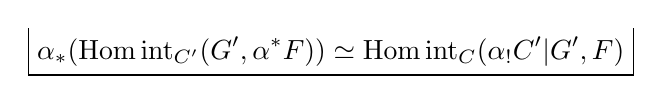
\begin{tikzpicture}[baseline=(eq.base)]
 \node[inner sep=3pt] (eq) {$\displaystyle\alpha_*(\mathrm{Hom\,int}_{C'}(G',\alpha^*F))\simeq
 \mathrm{Hom\,int}_{C}(\alpha_!\unsure{C'|G'},F)$};
 \draw (eq.north west)--(eq.south west)--(eq.south east)--(eq.north east);
 \end{tikzpicture}
\]
(\uline{Formule d'adjonction} ``\uline{interne}'', pour $\alpha_!$ et $\alpha^*$,
valable en principe pour \uline{\unsure{tte|tt}} $\alpha:C'\longrightarrow C$ dans $\mathrm{Diag}$. \unsure{tout} $G'$ dans $\mathbb D(C')$ et tout $F$ dans $\mathbb D(C)$.

Comment prouver cette formule ? En prenant l'opération produit $\otimes$, associée à l'\unsure{op|hop} Hom int, on est ramené \inserted{(en prenant les foncteurs contr. associés)} à une formule
\[
 G\otimes\alpha_!G'\xrightarrow{\sim}\alpha_!(\alpha^*\unsure{C|G}\otimes C')\unsure{,|/}
\]
\deleted{Si $G$ est de la forme $f^*G_0$ (\unsure{coeff|coeff.} \uline{constant} sur $C$)}

On trouve par adjonction un hom can $\unsure{-|\longrightarrow}$, il faut voir s'il est tjrs iso.
% archive sheet number: 152
